% License: CC BY-SA
% Authors: See authors below and see also acknowledgement for authors of some images or research

\documentclass[25pt, margin=0mm, innermargin=15mm, blockverticalspace=15mm, colspace=15mm, subcolspace=8mm]{tikzposter}
\geometry{paperwidth=197cm,paperheight=100cm}

% to stretch boxes over whole paper with custor paper size
\makeatletter
\setlength{\TP@visibletextwidth}{\textwidth-2\TP@innermargin}
\setlength{\TP@visibletextheight}{\textheight-2\TP@innermargin}
\makeatother


\usepackage[utf8]{inputenc}
\usepackage{wrapfig}
\usepackage[hidelinks]{hyperref}

% For blibliography styling
\usepackage{natbib}

\definecolor{titleTextColor}{HTML}{009000}
\definecolorpalette{grassColorPalette} {
  \definecolor{colorOne}{HTML}{419041}
}
\usecolorstyle[colorPalette=grassColorPalette]{Britain}

\title{
\Huge
\textcolor{titleTextColor}{
\textsf{\textbf{
\fontsize{85}{60}\selectfont
GRASS GIS: a peer-reviewed scientific platform and future research repository
}}
}
}

\newlength{\grasslogoheight}
\setlength{\grasslogoheight}{0.08\textheight}
\newlength{\instlogoheight}
\setlength{\instlogoheight}{0.45\grasslogoheight}

\titlegraphic{
\begin{minipage}{0.3\linewidth}

\includegraphics[height=\grasslogoheight]{grass}
~

\includegraphics[height=\grasslogoheight]{osgeo_project}
\end{minipage}
\hfill
\begin{minipage}{0.16\linewidth}
\setlength{\baselineskip}{120pt}
\begin{flushright}

\includegraphics[height=\instlogoheight]{iwmi}
~

\includegraphics[height=\instlogoheight]{ncstate}
~

\includegraphics[height=\instlogoheight]{ctu_prague}
~

\includegraphics[height=\instlogoheight]{fem_cri}
~

\includegraphics[height=\instlogoheight]{ec_jrc}
\end{flushright}
\end{minipage}
\vspace{-\grasslogoheight}
}

% \setlength{\blocktitleheight}{0.02\textheight}

% style for institute numbers
\newcommand{\inst}[1]{\hspace{2pt}$^{\mbox{\normalsize#1}}$\hspace{-7pt}}
\newcommand{\instlist}[1]{\hspace{1pt}$^{\mbox{\normalsize#1}}$\hspace{2pt}}

\author{
Yann Chemin\inst{2},
V\'{a}clav Petr\'{a}\v{s}\inst{1},
Anna Petr\'{a}\v{s}ov\'{a}\inst{1},
Martin Landa\inst{4},
S\"{o}ren Gebbert\inst{5},
Pietro Zambelli\inst{3},
Markus Neteler\inst{6}, and
Peter L\"{o}we\inst{7}
Margherita Di Leo\inst{8}
}
\institute{
\instlist{1}NCSU, USA,
\instlist{2}IWMI, Sri Lanka,
\instlist{3}EURAC, Italy,
\instlist{4}FCE CTU in Prague, Czech Republic,
\instlist{5}TICSA, Germany,
\instlist{6}CRI, FEM, Italy,
\instlist{7}GNLST, Germany
\instlist{8}EC-JRC, Italy
}

% \usetemplate{1}
% \setinstituteshift{1}

% \setblocktitleheight{2}
% \setblockspacing{1}

\graphicspath{{images/}{logos/}}

\newcommand{\blocktitlewrap}[1]{\textsf{\textbf{\huge#1}}}
% it is not possible (?) to change block title in the class, using wrapper
% the command introduced using:
%   sed -i 's/\\block{\([^}]*\)}/\\block{\\blocktitlewrap{\1}}/g' main.tex

% GRASS module
\newcommand{\gmodule}[1]{\href{http://grass.osgeo.org/grass70/manuals/#1.html}{\emph{#1}}}
\newcommand{\gamodule}[1]{\href{http://grass.osgeo.org/grass70/manuals/addons/#1.html}{\emph{#1}}}

\begin{document}
\maketitle[width=0.92\textwidth]
% \maketitle
% \addlogo[north west]{(2,-1)}{9cm}{images/Grass_GIS}
%Please insert your institution logo here
% \addlogo[north east]{(-2,-2.5)}{4cm}{images/logo_FEM_CRI}
% \addlogo[north east]{(-2,-5.5)}{4cm}{images/NC_State_Seal}
% \addlogo[north east]{(-8,-2.5)}{4cm}{images/Logo_cvut}
% \addlogo[north east]{(-8,-6.5)}{4cm}{images/IWMI_logo}
% \addlogo[north east]{(-2,-10.5)}{4cm}{images/logo_ec-jrc}

\begin{columns}

%%%%%%%%%%%%%%%%%%%%%%%%%%%%%%%%%%%%%%%%%%%%%%%%%%%%%%%%%%%%%%%%%%%%%
%%%%%%%%%%%%%%%%%%%%%%%%%%%%%%%%%%%%%%%%%%%%%%%%%%%%%%%%%%%%%%%%%%%%%
%%%%%%%%%%%%%%%%%%%%%%%%%%%%%%%%%%%%%%%%%%%%%%%%%%%%%%%%%%%%%%%%%%%%%
%%%%%%%%%%%%%%%%%%%%%%%%%%%%%%%%%%%%%%%%%%%%%%%%%%%%%%%%%%%%%%%%%%%%%
\column{0.25}

%%%%%%%%%%%%%%%%%%%%%%%%%%%%%%%%%%%%%%%%%%%%%%%%%%%%%%%%%%%%%%%%%%%%%%%%%%%%%%%%
\block{\blocktitlewrap{Introduction}}
{
Geographical Information Systems (GIS) are known for their capacity 
to spatially enhance the capacity of management of natural resources. 
While being often used as an analytical tool, they also represent a collaborative 
scientific platform to develop new algorithms. GRASS GIS (Neteler et al., 2012 
\cite{neteler2012grass}), a free and open source GIS, is used by many scientists 
directly or through other projects such as R or QGIS to perform geoprocessing tasks. 
Thus, a large number of scientific geospatial computations depend on quality and 
correct functionality of GRASS GIS. Integrating scientific algorithms into GRASS GIS 
helps to preserve reproducibility of scientific results over time as the original author 
designed it (Rocchini \& Neteler, 2012 \cite{rocchini2012let}). Moreover, subsequent 
improvements are tracked in the source code versioning system and are immediately 
available to the public (Petras, 2014 \cite{Petras2014}). Thus, GRASS GIS acts as a 
repository of scientific peer-reviewed code and algorithm/knowledge hub for future 
generation of scientists.
}

%%%%%%%%%%%%%%%%%%%%%%%%%%%%%%%%%%%%%%%%%%%%%%%%%%%%%%%%%%%%%%%%%%%%%%%%%%%%%%%%
\block{\blocktitlewrap{Landform detection: Geomorphons}}{

Jasiewicz and Stepinski \cite{jasiewicz2013geomorphons} developed a method and module \gamodule{r.geomorphon}
which provide orientation-invariant and relief-invariant method to classify landforms
in a scale-independent way.
Ashtekar et al. \cite{ashtekar2014digital} used geomorphons to study soil properties in northwestern South America.

\begin{minipage}{0.5\linewidth}
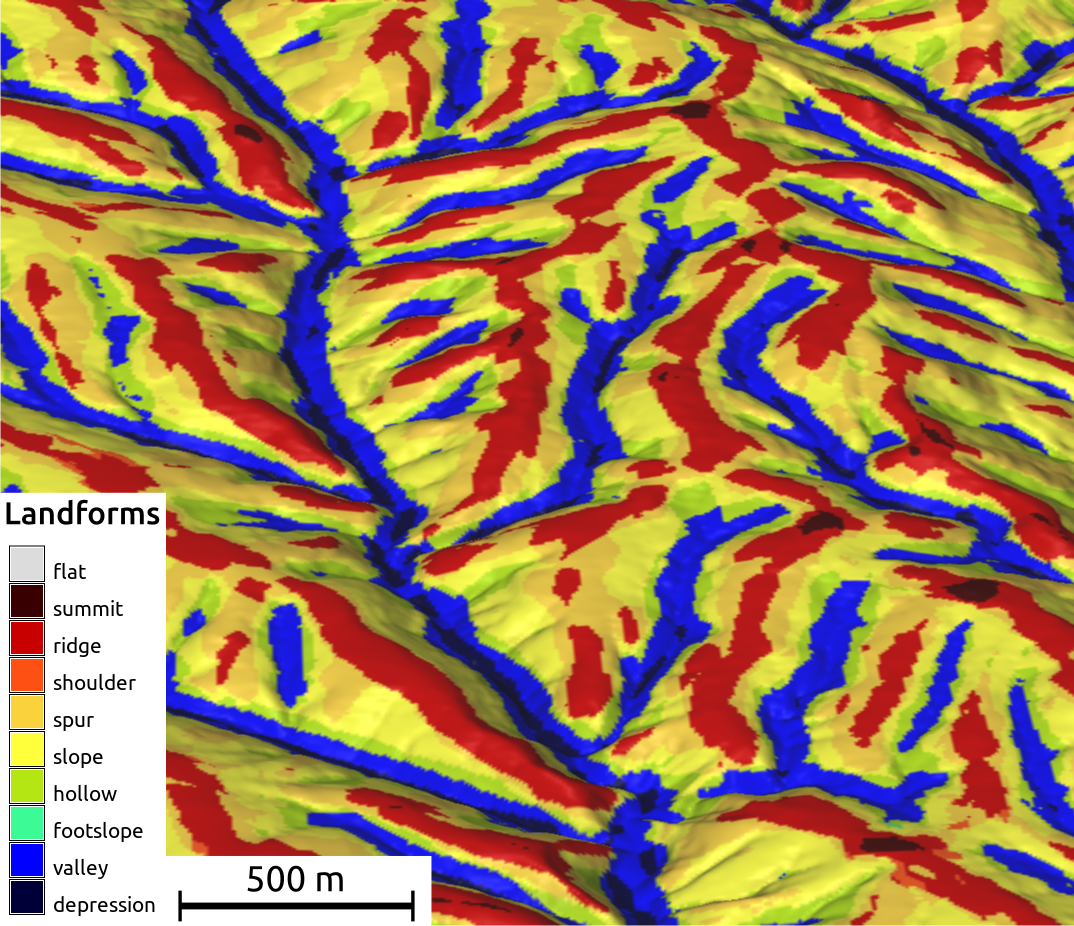
\includegraphics[width=\textwidth]{geomorphon}
Geomorphons for part of Yakima Training Center (area 5x3~km, USA)
\end{minipage}
~
\begin{minipage}{0.5\linewidth}
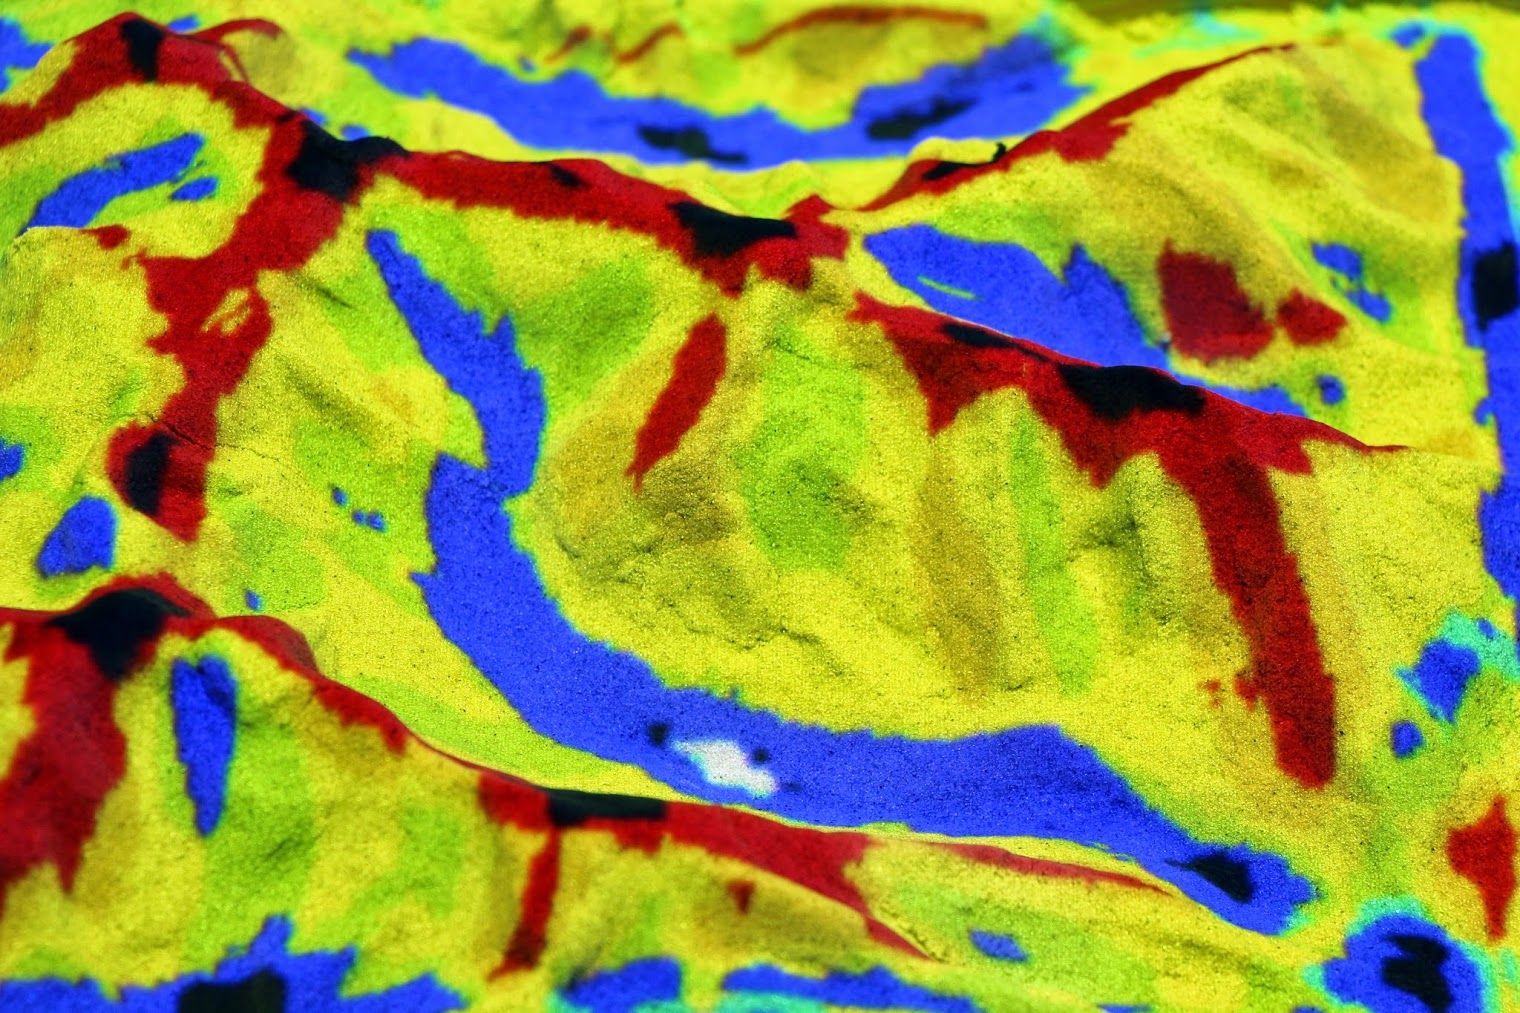
\includegraphics[width=\textwidth]{geomorphon_tangible_high_tatras}
Ridges and valleys detected on the sand physical model of High Tatras (Slovakia) using \gamodule{r.geomorphon} integrated in Tangible Landscape system
\end{minipage}
}


%%%%%%%%%%%%%%%%%%%%%%%%%%%%%%%%%%%%%%%%%%%%%%%%%%%%%%%%%%%%%%%%%%%%%%%%%%%%%%%%
\block{\blocktitlewrap{Natural Hazards: Wildfire Spread}}{
The wildfire simulation toolset, firstly developed by Xu, 1994 \cite{xu1994simulating}, 
implementing Rothermel’s model \cite{Rothermel1983how}, available through the GRASS 
functions \textit{r.ros} and \textit{r.spread}, is object of active research. It has been extensively 
tested and recently adapted to European fuel types (Rodriguez-Aseretto et al.,
2013 \cite{rodriguez2013data}; de Rigo et al., 2013 \cite{derigo2013architecture} ; 
Di Leo et al., 2013 \cite{2013_DiLeo_etAl}).

\begin{minipage}{0.5\linewidth}
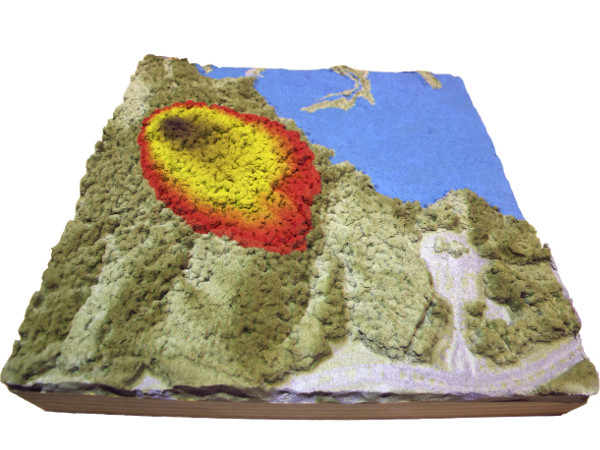
\includegraphics{fire}
Wildfire simulation in Tangible Landscape environment
\end{minipage}

\begin{minipage}{0.5\linewidth}
%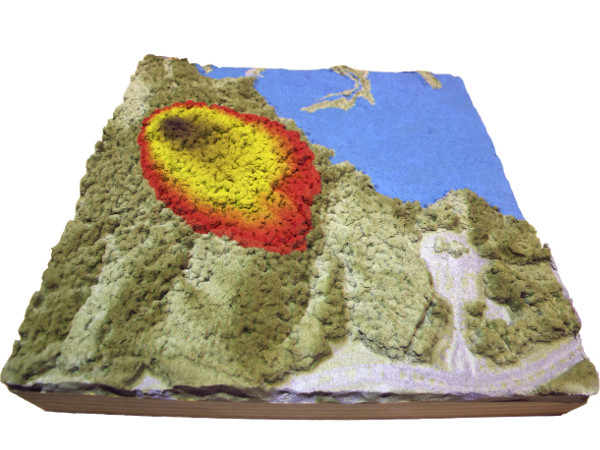
\includegraphics[width=\textwidth]{fire}
% TODO: Something from Europe
\end{minipage}
}

%%%%%%%%%%%%%%%%%%%%%%%%%%%%%%%%%%%%%%%%%%%%%%%%%%%%%%%%%%%%%%%%%%%%%
%%%%%%%%%%%%%%%%%%%%%%%%%%%%%%%%%%%%%%%%%%%%%%%%%%%%%%%%%%%%%%%%%%%%%
%%%%%%%%%%%%%%%%%%%%%%%%%%%%%%%%%%%%%%%%%%%%%%%%%%%%%%%%%%%%%%%%%%%%%
%%%%%%%%%%%%%%%%%%%%%%%%%%%%%%%%%%%%%%%%%%%%%%%%%%%%%%%%%%%%%%%%%%%%%
\column{0.25}


%%%%%%%%%%%%%%%%%%%%%%%%%%%%%%%%%%%%%%%%%%%%%%%%%%%%%%%%%%%%%%%%%%%%%%%%%%%%%%%
\block{\blocktitlewrap{Evapotranspiration (ET)}}{
With the various types of actual ET models being developed in the last 20 years, 
it becomes necessary to inter-compare methods. Most of already published ETa models 
comparisons address few number of models, and small to medium areas 
(Chemin, 2014 \cite{chemin2012distributed}; Gao and Long, 2008 \cite{gao2008intercomparison}; 
Garcia et al., 2007 \cite{garcia2007comparison}; Suleiman et al., 2008
\cite{suleiman2008intercomparison}; Timmermans et al., 2007 \cite{timmermans2007intercomparison}). 
With the large amount of remote sensing data covering the Earth, and the daily 
information available for the past ten years (i.e. Aqua/Terra-MODIS) for each pixel 
location, it becomes paramount to have a more complete comparison, 
in space and time.

To address this new experimental requirement, a distributed computing framework was 
designed, and created (Chemin, 2012 \cite{chemin2012distributed}). 
The design architecture was built from original satellite datasets to various levels 
of processing until reaching the requirement of various ETa models input dataset. 
Each input product is computed once and reused in all ETa models requiring such input. 
This permits standardization of inputs as much as possible to zero-in variations of 
models to the models internals/specificities. All of the ET models are available in the 
new GRASS GIS version 7 as imagery modules and replicability is complete for future 
research.

% TODO: images width captions
}

%%%%%%%%%%%%%%%%%%%%%%%%%%%%%%%%%%%%%%%%%%%%%%%%%%%%%%%%%%%%%%%%%%%%%
\block{\blocktitlewrap{Temporal framework (TGRASS)}}{

Described some applications

% TODO: images width captions
}

%%%%%%%%%%%%%%%%%%%%%%%%%%%%%%%%%%%%%%%%%%%%%%%%%%%%%%%%%%%%%%%%%%%%%
%%%%%%%%%%%%%%%%%%%%%%%%%%%%%%%%%%%%%%%%%%%%%%%%%%%%%%%%%%%%%%%%%%%%%
%%%%%%%%%%%%%%%%%%%%%%%%%%%%%%%%%%%%%%%%%%%%%%%%%%%%%%%%%%%%%%%%%%%%%
\column{0.25}

%%%%%%%%%%%%%%%%%%%%%%%%%%%%%%%%%%%%%%%%%%%%%%%%%%%%%%%%%%%%%%%%%%%%%%%%%%%%%%%%
\block{\blocktitlewrap{Natural Hazards: Water, Floods and Erosion}}{
GRASS GIS entails several modules that constitute the result of active research on 
natural hazard. The \gmodule{r.sim.water} simulation model (Mitas and Mitasova, 1998 \cite{Mitas1998b}) 
for overland flow under rainfall excess conditions was integrated into the Emergency 
Routing Decision Planning system as a WPS (Raghavan et al., 2014 \cite{raghavan2014deploying}). 
It was also modified by Petrasova et al., 2014 \cite{Petrasova2014} and is now part of a 
specialised software called \textit{Tangible Landscape} (previously \textit{Tangible GIS}), which also 
incorporated the \gamodule{r.damflood} module.

\begin{minipage}{0.5\linewidth}
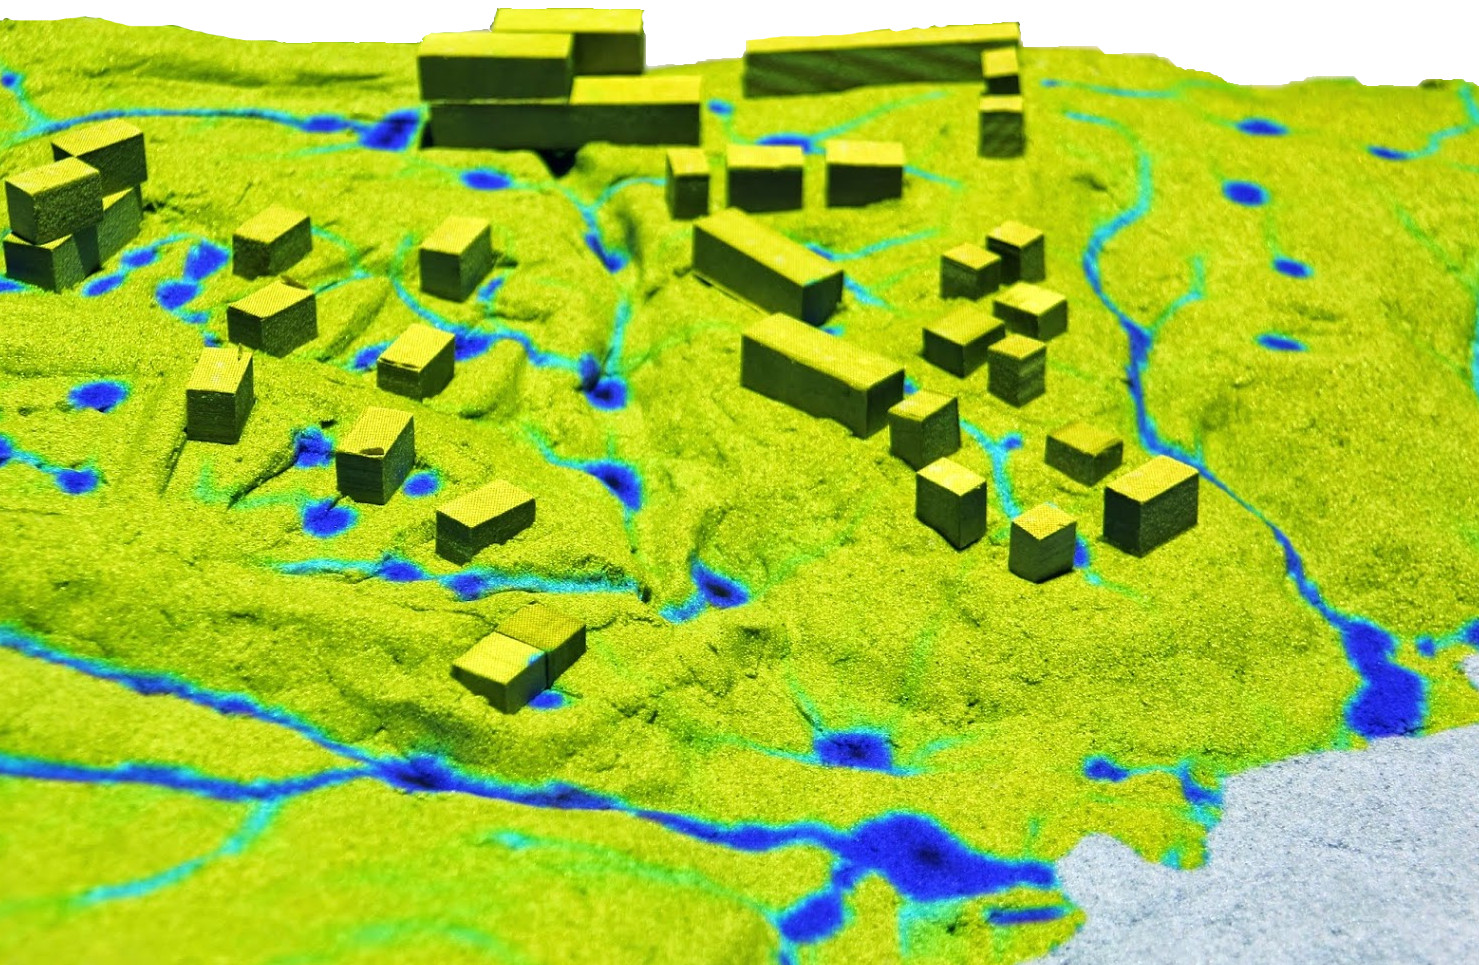
\includegraphics[width=\textwidth]{rsimwater_architects}
Overland flow used for landscape architecture design in Tangible Landscape environment
\end{minipage}
\begin{minipage}{0.5\linewidth}
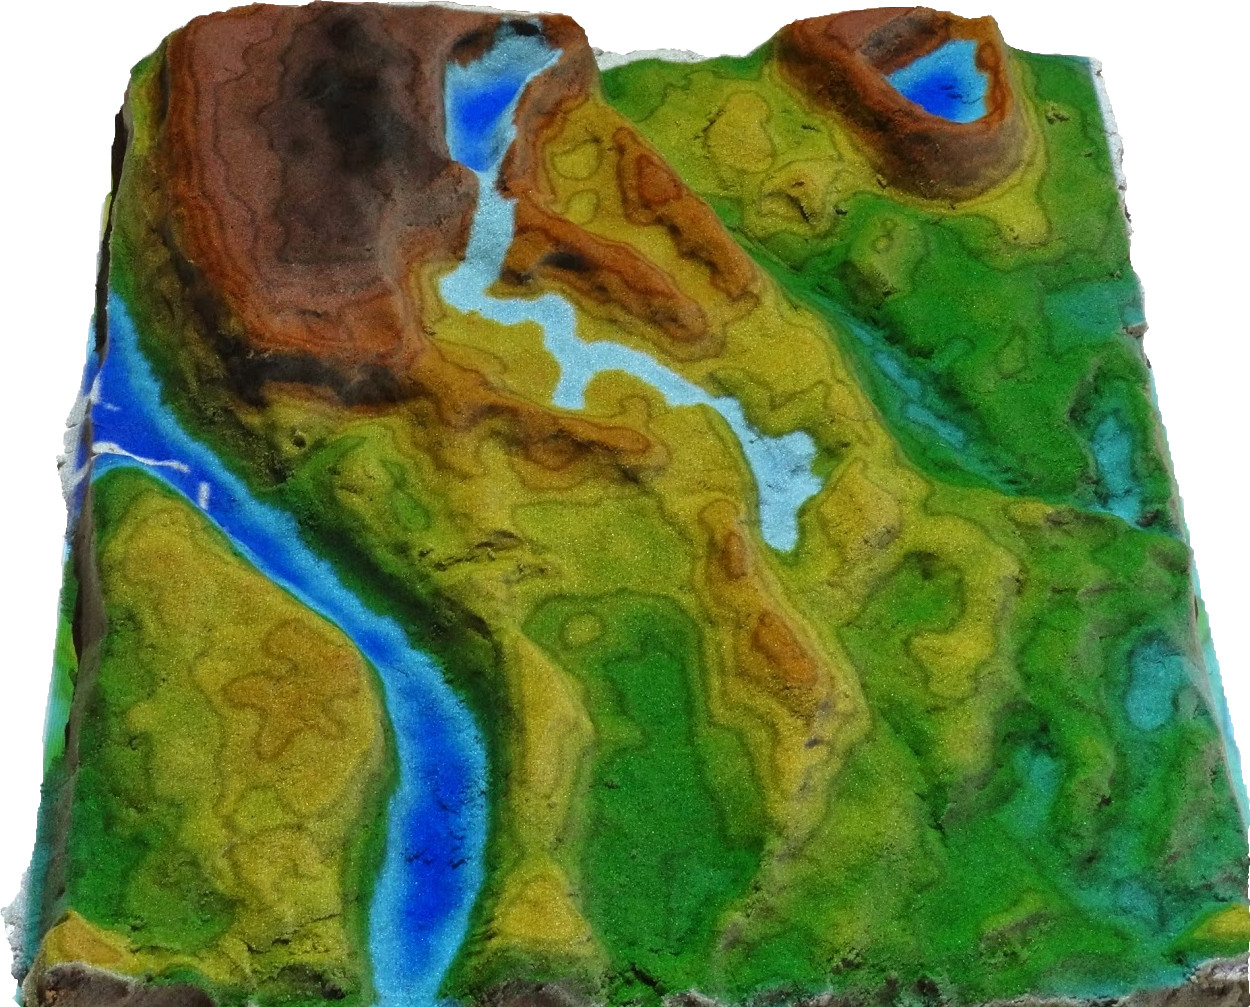
\includegraphics[width=\textwidth]{damflood_tangible}
Coal ash pond breach in Tangible Landscape environment using \gamodule{r.damflood} module
\end{minipage}
}


%%%%%%%%%%%%%%%%%%%%%%%%%%%%%%%%%%%%%%%%%%%%%%%%%%%%%%%%%%%%%%%%%%%%%%%%%%%%%%%%
\block{\blocktitlewrap{Spatial interpolation}}{
The module v.surf.rst for spatial interpolation was developed approximately 12 years 
ago, since then it was improved several times (Trac2, 2014). It is now an important part 
of GRASS GIS and is even taught at geospatial modeling courses, for example 
\url{http://courses.ncsu.edu/gis582/common/grass/interpolation_2.html}.
% TODO: move link to references

\begin{minipage}{0.5\linewidth}
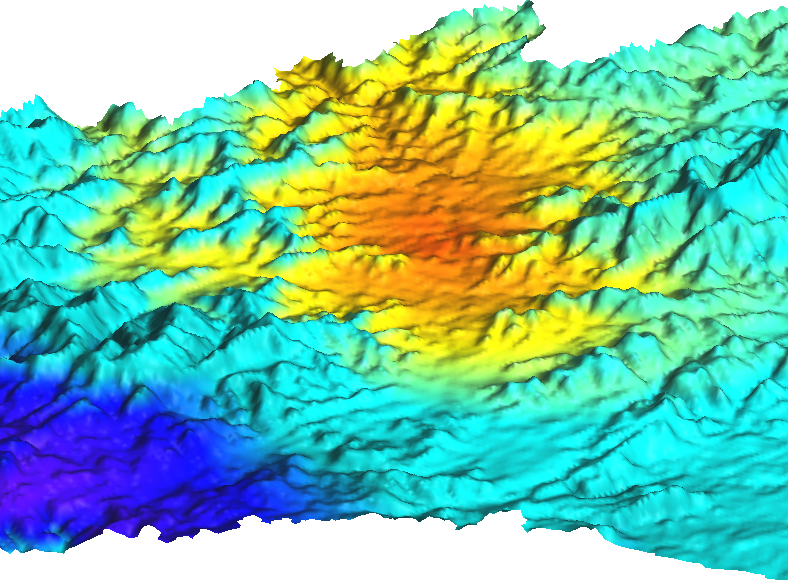
\includegraphics[width=\textwidth]{interpolation_precip_vvolrst}
Precipitation interpolated from meteorological stations in 3D space using \gmodule{v.vol.rst} in the area of North Carolina mountains (USA)
\end{minipage}
~
\begin{minipage}{0.5\linewidth}
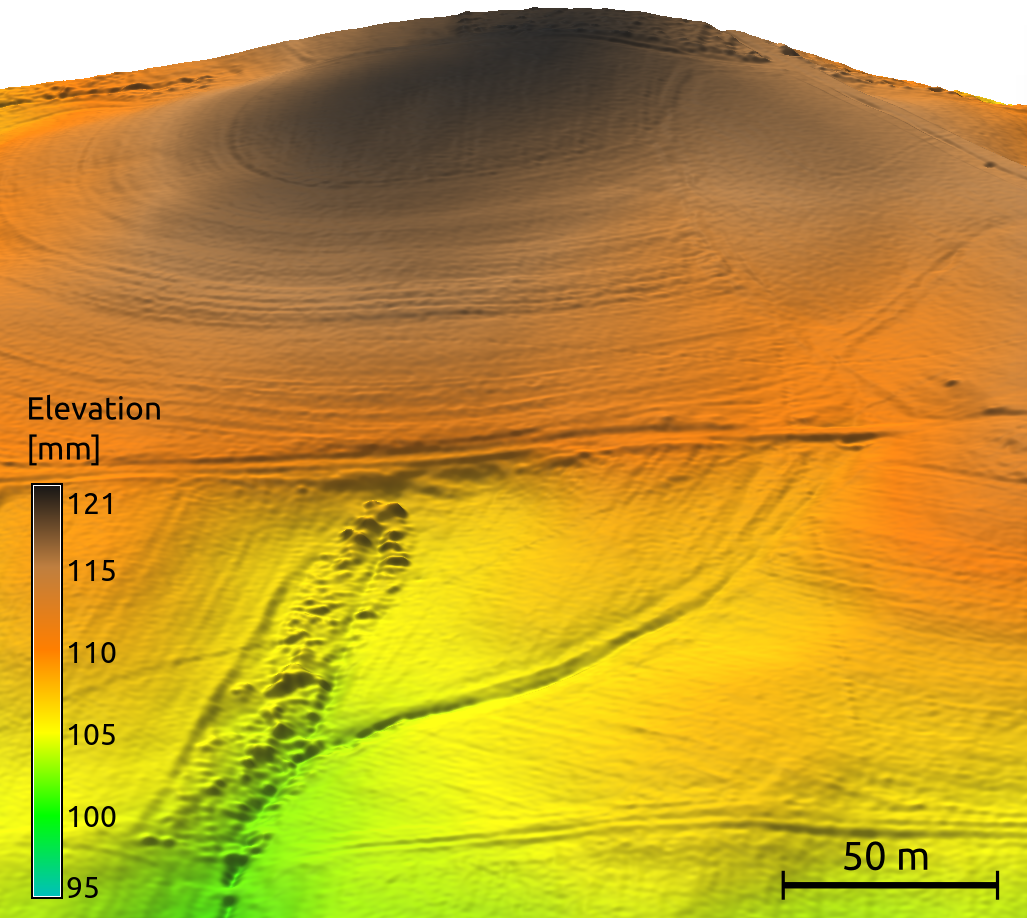
\includegraphics[width=\textwidth]{elevation_lidar}
Digital elevation model interpolated from lidar point cloud using \gmodule{v.surf.rst}. Data are showing tillage in an agricultural field near Raleigh (North Carolina, USA)
\end{minipage}
}

%%%%%%%%%%%%%%%%%%%%%%%%%%%%%%%%%%%%%%%%%%%%%%%%%%%%%%%%%%%%%%%%%%%%%
%%%%%%%%%%%%%%%%%%%%%%%%%%%%%%%%%%%%%%%%%%%%%%%%%%%%%%%%%%%%%%%%%%%%%
%%%%%%%%%%%%%%%%%%%%%%%%%%%%%%%%%%%%%%%%%%%%%%%%%%%%%%%%%%%%%%%%%%%%%
%%%%%%%%%%%%%%%%%%%%%%%%%%%%%%%%%%%%%%%%%%%%%%%%%%%%%%%%%%%%%%%%%%%%%
\column{0.25}

\block{\blocktitlewrap{Landscape structure}}{
A set of modules for multiscale analysis of landscape structure was added in 1992 
by Baker et al. \cite{baker1992r}, who developed the r.le model similar to 
FRAGSTATS \cite{mcgarigal1995fragstats}, see manual. The modules were gradually 
improved to become \textit{r.li} in 2006. Further development continued, with a significant 
speed up (Trac1, 2014) and new interactive user interface.
Rocchini et al. \cite{rocchini2013calculating} used \gmodule{r.li} modules to implement
high level tool for calculating landscape diversity.

\begin{minipage}{0.5\linewidth}
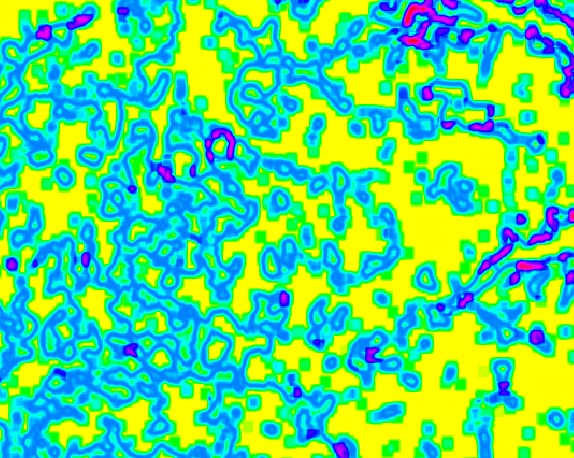
\includegraphics[width=\textwidth, trim={0 180 0 0}, clip]{rdiversity}
Landscape diversity according to shannon index in near Charlotte (North Carolina, USA).
\end{minipage}

% TODO: some other example or something completely else?
}

%%%%%%%%%%%%%%%%%%%%%%%%%%%%%%%%%%%%%%%%%%%%%%%%%%%%%%%%%%%%%%%%%%%%%%%%%%%%%%%
\block{\blocktitlewrap{Conclusions}}{
% TODO: review the points, it should be the highlight or something like that
% TODO: style of bullets is strange
\begin{itemize}
 \item Algorithms and models once included into GRASS GIS are still available.
 \item GRASS GIS development team takes care of API related updates and operating system related changes.
 \item Scientists are using highly specialized tools implemented by other people when having both scientific publication and source code at hand.
 \item New research and tools is build upon the existing one.
\end{itemize}
}


%%%%%%%%%%%%%%%%%%%%%%%%%%%%%%%%%%%%%%%%%%%%%%%%%%%%%%%%%%%%%%%%%%%%%%%%%%%%%%%%
\block{\blocktitlewrap{References and Acknowledgements}}{
\scriptsize

\newcommand{\blocksectiontitle}[1]{\subsubsection*{\textcolor{gray}{\textsf{#1}}}}

\blocksectiontitle{References}
\begingroup
\renewcommand{\section}[2]{}%
\bibliographystyle{plain}
\bibliography{poster}
\endgroup

\blocksectiontitle{Acknowledgements}
Matthew Horvath for \emph{Spill impacts from coal ash pond using GRASS GIS}
% http://www4.ncsu.edu/~jcfounta/Summer14Posters/horvath.pdf

Eva Stopkova for physical model of High Tatras.

GRASS GIS project is a Open Source Geospatial Foundation (OSGeo) project and is using OSGeo infrastructure for websites and repositories.

\textcolor{gray}{
\hrulefill
}
% \vspace{-5pt}

\newcommand{\qrcodesize}{0.05\linewidth}

% TODO: add proper QR codes and fix links

\begin{center}
\begin{tabular}{c}

% \hspace{5mm}

\begin{minipage}{\qrcodesize}

\includegraphics[width=\textwidth]{./images/grass_qr.pdf}
\end{minipage}

\begin{minipage}{0.15\linewidth}
\small {\url{grass.osgeo.org}}
\end{minipage}

\begin{minipage}{\qrcodesize}

\includegraphics[width=\textwidth]{./images/grass_qr.pdf}
\end{minipage}

\begin{minipage}{0.2\linewidth}
\small {\url{grasswiki.osgeo.org}}
\end{minipage}

\begin{minipage}{0.1\linewidth}
\href{http://creativecommons.org/licenses/by-sa/4.0/}{
\includegraphics[width=\textwidth]{ccbysa}}
\end{minipage}

\begin{minipage}{0.35\linewidth}
\small This poster is licensed under a Creative Commons Attribution-ShareAlike 4.0 International License.
\end{minipage}

\end{tabular}
\end{center}

}

\end{columns}

\end{document}
